\documentclass[12pt, a4paper, oneside, titlepage]{article}
\usepackage{amsmath,amssymb,amsfonts} % Typical maths resource packages
\usepackage{graphics}                 % Packages to allow inclusion of graphics
\usepackage{color}                    % For creating coloured text and background
\usepackage{hyperref}                 % For creating hyperlinks in cross references
\usepackage{enumerate}
\usepackage[utf8]{inputenc}
\usepackage[spanish]{babel}
\usepackage{epigraph}
\usepackage{calc}
\usepackage{multirow}
\usepackage[official]{eurosym}
\usepackage{listings}

\lstset{
  basicstyle=\ttfamily,
  columns=fullflexible,
  frame=single,
  breaklines=true,
  tabsize=2,
  postbreak=\mbox{\textcolor{red}{$\hookrightarrow$}\space},
}

%\usepackage[backend=biber,natbib=true,eprint=false,style=ieee,]{biblatex}
%natbib=true,
%url=false, 
%doi=true,
%eprint=false
%\addbibresource{database.bib}


\newcommand{\mytextformat}{\itshape\epigraphsize}
\newenvironment{mytext}{\mytextformat}{}
\newenvironment{mysource}{\scshape\hfill}{}
\renewcommand{\textflush}{mytext} 
\renewcommand{\sourceflush}{mysource}

\let\originalepigraph\epigraph 
\renewcommand\epigraph[2]%
{\setlength{\epigraphwidth}{\widthof{\mytextformat#1}}\originalepigraph{#1}{#2}}

%\usepackage{titlesec}
\usepackage{tocloft}
\renewcommand{\cftsecleader}{\cftdotfill{\cftdotsep}}
\usepackage{lipsum}
%\usepackage{makeidx}
\usepackage{color}   %May be necessary if you want to color links
\usepackage{hyperref}
\hypersetup{
	colorlinks=true, %set true if you want colored links
	linktoc=all,     %set to all if you want both sections and subsections linked
	linkcolor=black,  %choose some color if you want links to stand out
}
\usepackage[pdftex]{graphicx}

\newcommand{\HRule}{\rule{\linewidth}{0.5mm}}

\setlength{\parindent}{2em}
\setlength{\parskip}{1em}

\usepackage{float}
\newcommand{\separador}{\subsubsection*{} \noindent}

\pagestyle {myheadings}

\begin{document}
	
	\begin{titlepage}
		\begin{center}
			\textsc{\LARGE }\\[1.5cm]
			\textsc{\Large }\\[0.5cm]
			Deutsches Zentrum für Luft- und Raumfahrt\\
			Experimental Gravitational Physics and Geodesy \\
			\HRule \\[0.8cm]
			{ \huge \bfseries Instalación y puesta en marcha de sistema de interfaz visual.}\\[0.4cm]
			
\begin{Large}
						Con simplificación de sensores de temperatura y luz

			\end{Large}			\HRule \\[1.5cm]
			
			% Author and supervisor
			\begin{minipage}{0.4\textwidth}
				\begin{flushleft} \large
					\emph{Autor:}\\
					Pablo \textsc{Torres Anaya}
				\end{flushleft}
			\end{minipage}
			\begin{minipage}{0.4\textwidth}
				\begin{flushright} \large
					%\emph{Ilustradora:} \\
					%Rocio \textsc{}
				\end{flushright}
			\end{minipage}
			\vfill
			%\includegraphics[width=25mm]{cc.jpg} \\
			%Esta obra está bajo una \href{http://creativecommons.org/licenses/by-nc-nd/3.0/deed.es}{Licencia Creative Commons Atribución-NoComercial-SinDerivadas 3.0 Unported.}\\
			{\large \today}\\
			{\normalsize Powered by \LaTeX}
			
		\end{center}
	\end{titlepage}
	%Esquema general
	\tableofcontents
%%%%%%%
%SECTION
%%%%%%%
\begin{abstract}
Para el siguiente documento se considera que tenemos una raspberrypi con Raspian instalado y todo el desarrollo se hace en local (la propia raspberrypi)
%TODO 
Poner algún resumen del contenido del documento
--todo--
\end{abstract}
\section{Preparación RaspberryPi}

%SUB-SECTION
\subsection{Instalación de software}

\subsubsection{MQTT}

Para instalar mqtt en linux (raspbery) debemos ejecutar en la consola:
\begin{lstlisting}[frame=single]
sudo apt-get install mosquitto
 \end{lstlisting}
Si queremos tener clientes mosquitto en la raspberry (para testing) ponemos:
\begin{lstlisting}[frame=single]
sudo apt-get install mosquitto-clients
 \end{lstlisting}
 
Para poder usar mqtt desde python, en los scripts tenemos que ejecutar:
\begin{lstlisting}[frame=single]
pip install paho-mqtt
\end{lstlisting}
 
 En caso de no tener pip, tenemos que instalarlo:
\begin{lstlisting}[frame=single]
 sudo apt-get install python-pip
 \end{lstlisting}

Con esto ya tenemos la estructura básica para capturar datos desde los dispositivos y mandarlos al broker mqtt.

\subsubsection{Influx + Grafana}

Para instalar grafana e influx he seguido el siguiente tutorial:
http://engineer.john-whittington.co.uk/2016/11/raspberry-pi-data-logger-influxdb-grafana/

(copio las líneas importantes en caso de que la url se pierda:)
 
Instalación:
\begin{lstlisting}[frame=single]
# update these URLs by looking at the website: https://packages.debian.org/sid/grafana
sudo apt-get update
sudo apt-get upgrade
wget http://ftp.us.debian.org/debian/pool/main/i/influxdb/influxdb_1.0.2+dfsg1-1_armhf.deb
sudo dpkg -i influxdb_1.0.2+dfsg1-1_armhf.deb
wget http://ftp.us.debian.org/debian/pool/main/g/grafana/grafana-data_2.6.0+dfsg-3_all.deb # grafana data is a dependancy for grafana
sudo dpkg -i grafana-data_2.6.0+dfsg-3_all.deb
sudo apt-get install -f
wget http://ftp.us.debian.org/debian/pool/main/g/grafana/grafana_2.6.0+dfsg-3_armhf.deb
sudo dpkg -i grafana_2.6.0+dfsg-3_armhf.deb
sudo apt-get install -f
 
 \end{lstlisting}

Con eso deberíamos tener instalados Influx y Grafana.

Para usar influx desde python (Necesario para guardar los datos desde el script principal:
 
\begin{lstlisting}
sudo pip install influxdb
 \end{lstlisting}
 

 Por ultimo activamos Grafana para que esté disponible en cada arranque:
 
\begin{lstlisting}
sudo systemctl enable grafana-server
sudo systemctl start grafana-server
\end{lstlisting}
 




\subsubsection{Node-Red}

Node-Red debería venir instalado por defecto en nuestra Raspberry si usamos Raspian. Pero en caso de no tenerlo podemos instalarlo ejecutando lo siguiente:

\begin{lstlisting}[frame=single]
bash <(curl -sL https://raw.githubusercontent.com/node-red/raspbian-deb-package/master/resources/update-nodejs-and-nodered)
\end{lstlisting}

Si ya lo tenemos pre-instalado se recomienda actualizarlo antes de empezar a usarlo:

\begin{lstlisting}[frame=single]
$ update-nodejs-and-nodered
\end{lstlisting}

Una vez instalado tenemos que ejecutarlo:
\begin{lstlisting}[frame=single]
$ node-red
\end{lstlisting}

y acceder a su url localhost:1880
y ya podemos empezar a usarlo.

Instalación de sub-módulos:

Dashboard:
To install the stable version run the following command in your Node-RED user directory (typically ~/.node-red):

\begin{lstlisting}[frame=single]
$ npm i node-red-dashboard
\end{lstlisting}

Telegram Integration:
\begin{lstlisting}[frame=single]
npm i node-red-contrib-telegrambot
\end{lstlisting}

\subsubsection{Script-Python}

Descargar/clonar repositorio.

Para tener la ultima versión estable del script se recomienda clonar el repositorio en la rama 'Release'. 
Pero para poder clonar el repositorio 'cómodamente' tenemos que dar acceso a la raspberry al repositorio. Esto hay que hacerlo mientras tengamos el código en Bitbucket, cuando lo tengamos listo para funcionar lo podemos guardar en una plataforma de acceso mas cómoda.

Para hacerlo hay que generar un par de claves pública-privada y agregar la clave pública a Bitbucket. Para ello seguimos los pasos detallados en \url{https://confluence.atlassian.com/bitbucket/set-up-ssh-for-git-728138079.html}. Los cuales resumo a continuación:

Comprobamos las keys actuales del sistema (para no pisar nombres).


sudo pip3 install pyserial

\begin{lstlisting}
$ ls -a ~/.ssh
\end{lstlisting}
Generamos una nueva pareja de claves.

\begin{lstlisting}
$ ssh-keygen 
\end{lstlisting}

Comprobamos que se han generado bien.
\begin{lstlisting}
$ ls -a ~/.ssh
\end{lstlisting}

Comprobar si el agente sh está ejecutándose:
\begin{lstlisting}
$ ps -e | grep [s]sh-agent
 9060 ?? 0:00.28 /usr/bin/ssh-agent -l
\end{lstlisting}

Si no se está ejecutando lo arrancamos
\begin{lstlisting}
$ ssh-agent /bin/bash
\end{lstlisting}

Agregamos el id\_rsa generado (o el nombre que le pusiéramos al principio)
Recomiendo no poner contraseña al fichero.
\begin{lstlisting}
$ ssh-add ~/.ssh/id_rsa
\end{lstlisting}

Comprobamos que está agregada correctamente.
\begin{lstlisting}
$ ssh-add -l 
\end{lstlisting}

Extraemos el id publico que es el que hay que agregar a Bitbucket. 
\begin{lstlisting}
$ cat ~/.ssh/id_rsa.pub
\end{lstlisting}

Pasar el resultado al Administrador del repositorio (a fecha de hoy: Pablo Torres) para que agregue ese id a la lista de acceso. 

Una vez estamos autorizados podemos clonar el repositorio ejecutando:

\begin{lstlisting}
$ git clone git@bitbucket.org:dlrgeodesy/raspberry.git
$ cd raspberry
$ git fetch && git checkout Release
\end{lstlisting}

Con eso ya estamos listos para ejecutar el script de python.

%SUB-SECTION
\subsection{Configuración}
%TODO 
%un pequeño resumen
--todo-- pequeño resumen

\subsubsection{Influx}

 
conectándose a http://localhost:8083 desde la raspberry accedemos al panel de control donde podemos crear una base de datos.  (El usuario y password por defecto es admin/admin)


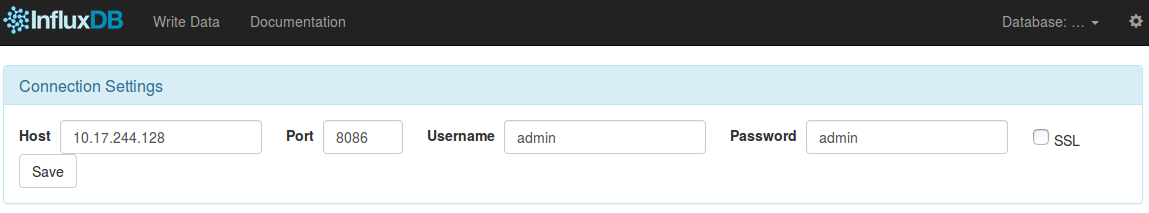
\includegraphics[width=0.9\linewidth,keepaspectratio]{img/influx_1.png}

Para crear una ''Base de datos'' en Influx escribimos en la interface: (sustituyendo ''db\_name'' por el nombre que queramos darle a la base de datos, en este ejemplo y posteriores)

\begin{lstlisting}
CREATE DATABASE "db_name"
\end{lstlisting}
 
Una vez tenemos la ''Database'' hay que entender que las tablas (MEASUREMENTS) se generan dinámicamente cuando hacemos los ''inserts'', y no tienen que ser declaras (ni sus columnas) 
 
Pero nos queda una cosa mas por hacer: Modificar la política de retención que genera por defecto por la que proporciona la plantilla de la interface. Para que los datos se guarden el tiempo que queramos.

Para ello primero borramos la política por defecto:

\begin{lstlisting}
DROP RETENTION POLICY "autogen" ON "db_name"
\end{lstlisting}
Ahora generamos una con los parametros que queremos:

\begin{lstlisting}
CREATE RETENTION POLICY "rp_name" ON "db_name" DURATION 30d REPLICATION 1 DEFAULT
\end{lstlisting}

Ya estamos listos para guardar valores en la base de datos que hemos creado. Es importante apuntar el nombre porque vamos a tener que usarlo mas adelante.

\subsubsection{Grafana}


Accediendo a la url localhost:3000 accedemos a grafana. Nos pide un login que es admin/admin
En Datasource debemos configurar la base de datos influx, usando los parámetros de conexión necesarios y el nombre de la base de datos que hemos creado previamente. Y si todo va bien ya está todo listo para recibir y pintar datos.
%TODO
--todo-- poner captura y query

\subsubsection{Node-Red}

A priori no necesita configuración adicional. La creación/uso de los nodos no los considero configuración, por lo que los veremos en el ultimo apartado. Ya que es algo dinámico que nos va a permitir ajustar el funcionamiento del sistema on-line.

Y para esto hay infinidad de tutoriales/guías que en caso de querer profundizar mas en el tema recomiendo buscarlos.

\subsubsection{Script-Python}

Por simplicidad y comodidad, toda la explicación del funcionamiento y uso del fichero de configuración JSON del script de python, se puede encontrar en otro documento (Doc\_Json.pdf) 


%SUB-SECTION
\subsection{Pautas de Funcionamiento}
%TODO 
Explicar como conectar a grandes rasgos los dispositivos y un resumen del flujo de trabajo.
Que hacer primero y como preparar las cosas
--todo--


%%%%%%%
%SECTION
%%%%%%%
\section{Tutorial de uso - Cohete}
%TODO 

\subsection{Arduino}
%TODO H

Hacer un resumen del apartado y explicar el proyecto del cohete.
--todo--


%SUB-SECTION
\subsubsection{Circuito}
%TODO 

%TODO: Revisar que estas sean las conexiones correctas
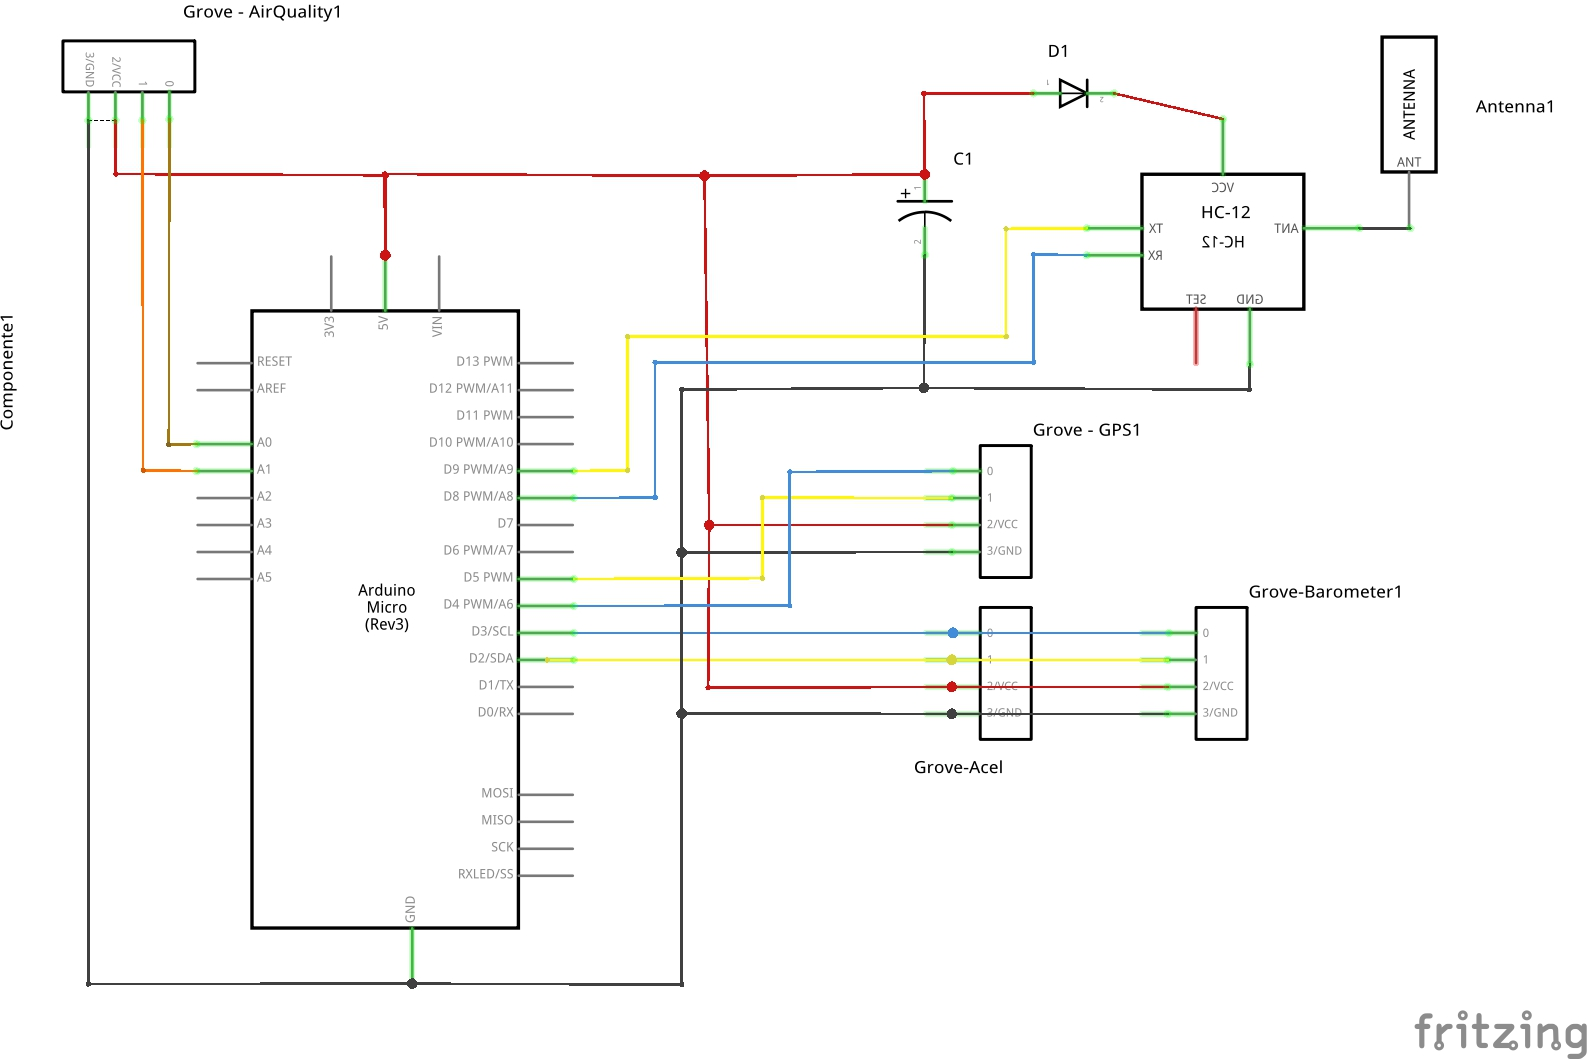
\includegraphics[width=0.9\linewidth,keepaspectratio]{img/RocketSketch_schem.jpg}

Explicar el circuito al detalle
--todo--


%SUB-SECTION
\subsubsection{Código}
%TODO 
(Poner solo las partes que no son librerías) y enlaces de descarga de las librerías
--todo--
\subsection{Script Python}
%TODO 
Ejemplo de uso desde 0 del script para el cohete

\begin{lstlisting}
{
	"control": {
		"address": "localhost",
		"port": 1883,
		"topic": "master/control",
		"qos": 0,
		"control_messages": {
			"reload": "reload",
			"shutdown": "shutdown",
			"status": "status"
		}
	},
	"dbs": {
		"db0":{
			"id_deprecated": "db0",
			"class_name": "Influx",
			"addres": "localhost",
			"port": "default",
			"db_name": "payload_logger",
			"user": "admin",
			"password": "admin"
		}
	},
	"joiners": {
		"join_1":{
			"function": "(abs{0}+abs{1}+abs{2})",
			"topics": {
			  "raw_all":  {
					"function": "Raw",
					"samples": 1,
					"topic": "rocket/acelerometer/all",
					"to_db":{
						"table":"rocket/acelerometer/all",
						"column":"payload",
						"db_id":"db0"
					}
				}
			}
		}
	},
	"sockets": {

		"id_serialsocket_rocket": {
			"class_name": "SerialSocket",
			"eol_character":";",
			"publish": {
				"parser": "#{0},{1},{2}:{3},{4},{5}:{6},{7},{8}:{9};",
				"join": [
					{
						"from": "0",
						"to": "join_1",
						"position": 0
					},
					{
						"from": "1",
						"to": "join_1",
						"position": 1
					},{
						"from": "2",
						"to": "join_1",
						"position": 2
					}
				],

				"topics": {
					"0": {
						"raw":{
							"function": "Raw",
							"samples": 1,
							"topic": "rocket/acelerometer/x",
							"to_db":{
								"table":"rocket/acelerometer/x",
								"column":"payload",
								"db_id":"db0"
							}
						},
						"mean":{
							"function": "Mean",
							"samples": 10,
							"topic": "rocket/acelerometer/x/mean"
						}
					},
					"1": {
						"raw":{
							"function": "Raw",
							"samples": 1,
							"topic": "rocket/acelerometer/y",
							"to_db":{
								"table":"rocket/acelerometer/y",
								"column":"payload",
								"db_id":"db0"
							}
						},
						"mean":{
							"function": "Mean",
							"samples": 10,
							"topic": "rocket/acelerometer/y/mean"
						}
					},
					"2": {
						"raw":{
							"function": "Raw",
							"samples": 1,
							"topic": "rocket/acelerometer/z",
							"to_db":{
								"table":"rocket/acelerometer/z",
								"column":"payload",
								"db_id":"db0"
							}
						},
						"mean":{
							"function": "Mean",
							"samples": 10,
							"topic": "rocket/acelerometer/z/mean"
						}
					},
					"3": {
						"raw":{
							"function": "Raw",
							"samples": 1,
							"topic": "rocket/varometer/temperature",
							"to_db":{
								"table":"rocket/varometer/temperature",
								"column":"payload",
								"db_id":"db0"
							}
						},
						"mean":{
							"function": "Mean",
							"samples": 10,
							"topic": "rocket/varometer/temperature/mean"
						}
					},
					"4": {
						"raw":{
							"function": "Raw",
							"samples": 1,
							"topic": "rocket/varometer/presion",
							"to_db":{
								"table":"rocket/varometer/presion",
								"column":"payload",
								"db_id":"db0"
							}
						},
						"mean":{
							"function": "Mean",
							"samples": 10,
							"topic": "rocket/varometer/presion/mean"
						}
					},
					"5": {
						"raw":{
							"function": "Raw",
							"samples": 1,
							"topic": "rocket/varometer/altitude",
							"to_db":{
								"table":"rocket/varometer/altitude",
								"column":"payload",
								"db_id":"db0"
							}
						},
						"mean":{
							"function": "Mean",
							"samples": 10,
							"topic": "rocket/varometer/altitude/mean"
						}
					},
					"6": {
						"raw":{
							"function": "Raw",
							"samples": 1,
							"topic": "rocket/gps/latitude",
							"to_db":{
								"table":"rocket/gps/latitude",
								"column":"payload",
								"db_id":"db0"
							}
						},
						"mean":{
							"function": "Mean",
							"samples": 10,
							"topic": "rocket/gps/latitude/mean"
						}
					},
					"7": {
						"raw":{
							"function": "Raw",
							"samples": 1,
							"topic": "rocket/gps/longitude",
							"to_db":{
								"table":"rocket/gps/longitude",
								"column":"payload",
								"db_id":"db0"
							}
						},
						"mean":{
							"function": "Mean",
							"samples": 10,
							"topic": "rocket/gps/longitude/mean"
						}
					},
					"8": {
						"raw":{
							"function": "Raw",
							"samples": 1,
							"topic": "rocket/gps/altitude",
							"to_db":{
								"table":"rocket/gps/altitude",
								"column":"payload",
								"db_id":"db0"
							}
						},
						"mean":{
							"function": "Mean",
							"samples": 10,
							"topic": "rocket/gps/altitude/mean"
						}
					},
					"9": {
						"raw":{
							"function": "Raw",
							"samples": 1,
							"topic": "rocket/airquality/value",
							"to_db":{
								"table":"rocket/airquality/value",
								"column":"payload",
								"db_id":"db0"
							}
						},
						"mean":{
							"function": "Mean",
							"samples": 10,
							"topic": "rocket/airquality/value/mean"
						}
					}
				}
			},
			"port": "/dev/ttyACM0",
			"baudrate":9600,
			"delay": 0
		}
	}

}
\end{lstlisting}
--todo--
\subsection{Influx + Grafana}
Lo primero que tenemos que hacer es conectarnos a influx localhost:8083 y configurar el usuario y contraseña de la sesión tal como se muestra en la captura. Una vez introducido los datos le damos a "save" y si todo está correcto tenemos acceso a la base de datos.

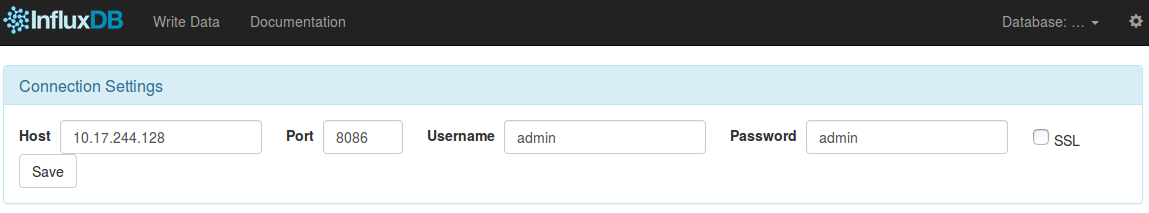
\includegraphics[width=0.9\linewidth,keepaspectratio]{img/influx_1.png}

Ahora procedemos a crear la base de datos si no la habíamos creado y no hay que olvidar cambiarle la RetentionPolicy.

Y ya estamos listos para almacenar datos y verlos en Influx. Dado que las tablas y columnas se crean dinámicamente.

Para visualizar los datos desde influx podemos ejecutar la siguiente query:

\begin{lstlisting}
SELECT "payload" FROM "rocket/acelerometer/all"
\end{lstlisting}

Ahora vamos a preparar las gráficas de grafana para que muestren los datos que nos interesan. En nuestro caso vamos a mostrar solo la suma de las aceleraciones, pero para el resto de medidas es simplemente repetir el proceso.

Lo primero es asegurarnos de que está / crear el datasource para la DB ''logger''. Como podemos ver en la siguiente captura.

Tenemos que tener en cuenta que la url es relativa a grafana. Es decir, si se ejecutan en la misma máquina la url será localhsot, aunque nosotros estemos accediendo mediante otra dirección.

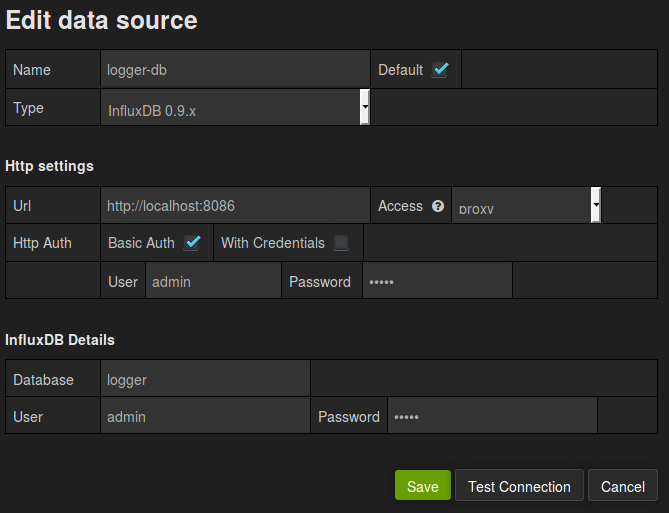
\includegraphics[width=0.9\linewidth,keepaspectratio]{img/grafana-1.png}

Ahora que tenemos el ''Datasource'' listo, podemos usarlo para crear un dashboard.

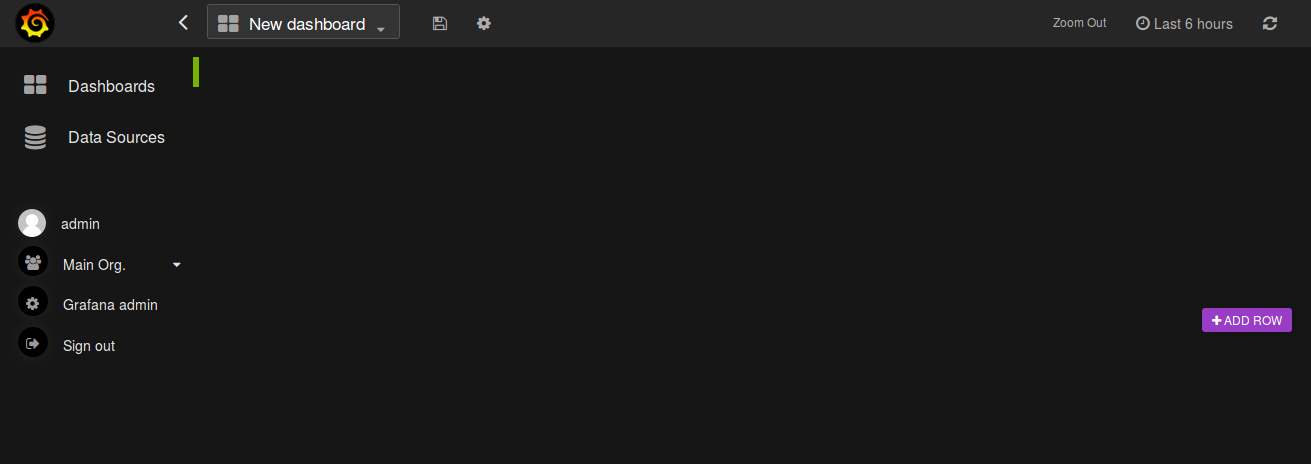
\includegraphics[width=0.9\linewidth,keepaspectratio]{img/grafana-2.png}

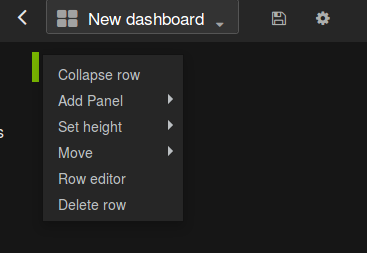
\includegraphics[width=0.9\linewidth,keepaspectratio]{img/grafana-3.png}

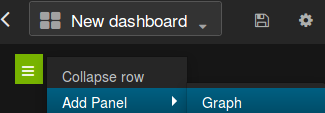
\includegraphics[width=0.9\linewidth,keepaspectratio]{img/grafana-4.png}

Ahora agregamos la query que queremos y en cuanto empecemos a introducir datos en la base de datos deberían verse los puntos.

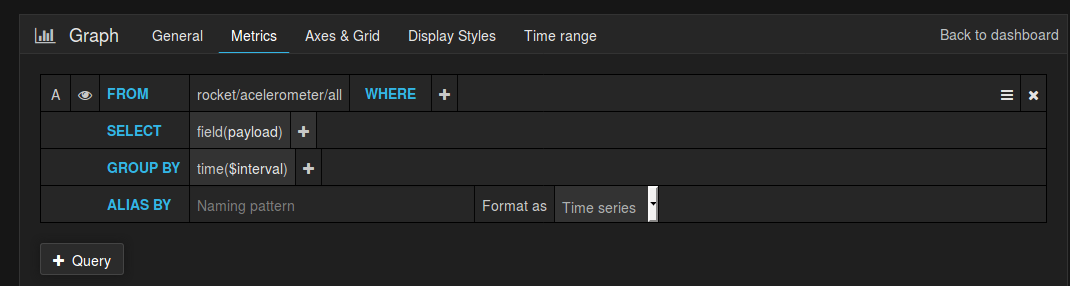
\includegraphics[width=0.9\linewidth,keepaspectratio]{img/grafana-5.png}

\subsection{Node-Red}
%TODO 
%Ejemplo de uso desde 0 de un flujo de 'ploteo' y control de node-red

Primero nos conectamos a Node-Red en la dirección localhost:1880. 

Si es la primera vez que conectamos tendremos la ventana del flow1 en blanco donde podemos empezar a trabajar directamente. En caso contrario podemos crear un flow nuevo para el propósito de este ejemplo.

El sistema de programación/uso de Node-Red es mediante la colocación de nodos y su interconexión.

A continuación imagen a imagen vamos a ver la creación de un flujo sencillo para mostrar los datos del cohete.

Primero creamos un nodo de entrada MQTT y lo configuramos

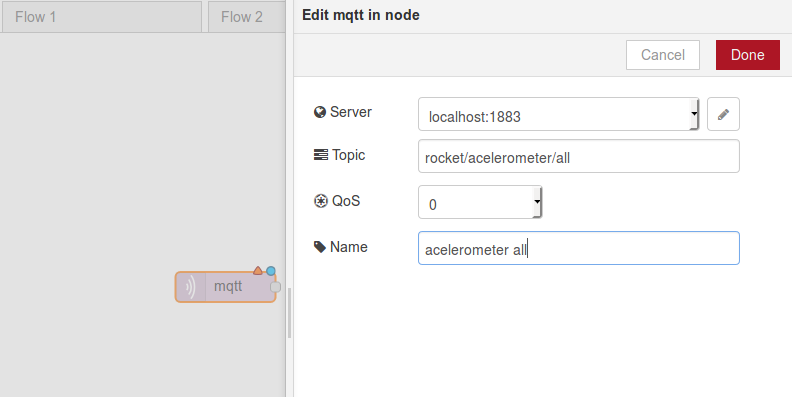
\includegraphics[width=0.9\linewidth,keepaspectratio]{img/node-1.png}

Después creamos un nodo de salida Gráfica y lo configuramos

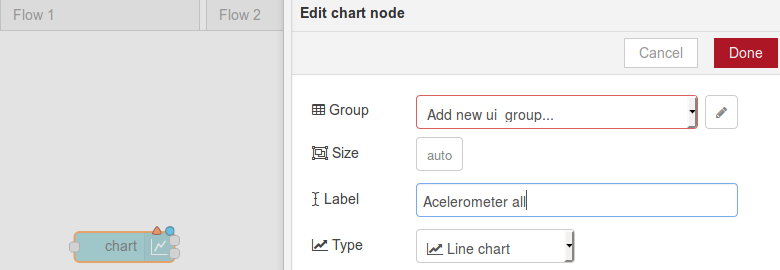
\includegraphics[width=0.9\linewidth,keepaspectratio]{img/node-2.png}

Le tenemos que crear un grupo y una tabla en el dashboard

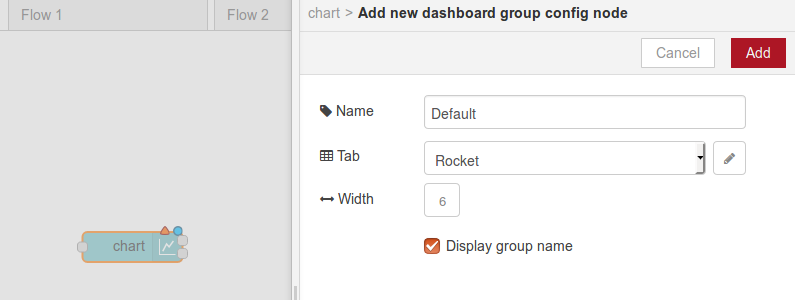
\includegraphics[width=0.9\linewidth,keepaspectratio]{img/node-3.png}

Y después los conectamos

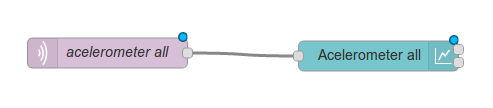
\includegraphics[width=0.9\linewidth,keepaspectratio]{img/node-4.png}

Repitiendo el proceso podemos crear sistemas complejos.
En la pestaña de info a la derecha tenemos una información muy completa de como funciona cada nodo cuando lo seleccionamos. Suena a tópico pero el límite es nuestra imaginación (y la capacidad de computo del pc)

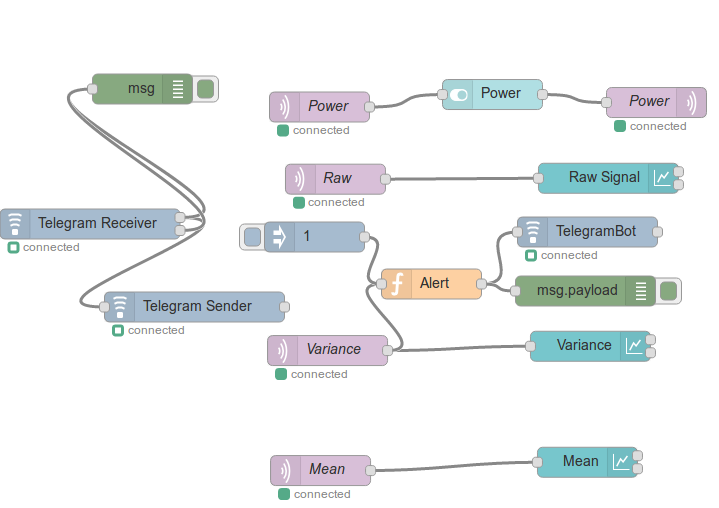
\includegraphics[width=0.9\linewidth,keepaspectratio]{img/node-5.png}

Para incluir grafana dentro de node red le creamos un enlace. Hay que tener en cuenta que la dirección que debemos introducir en el enlace es relativa a nuestra máquina. Es decir, debe ser la misma que usaríamos para acceder nosotros mismos a grafana. 

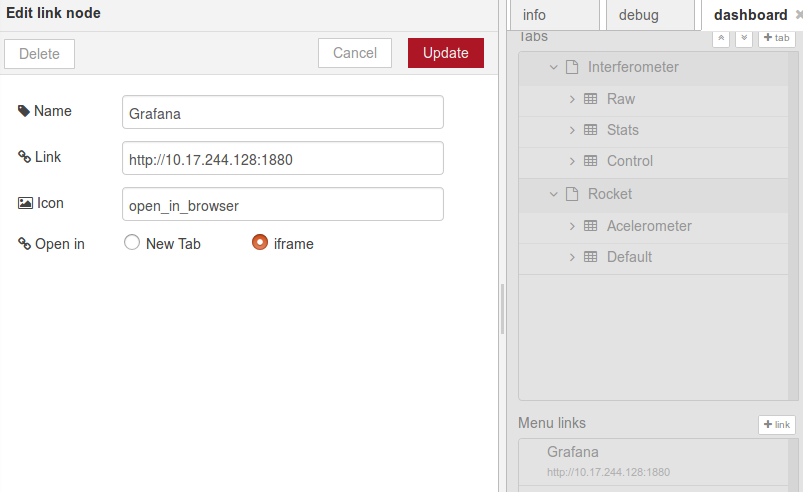
\includegraphics[width=0.9\linewidth,keepaspectratio]{img/node-6.png}


\subsection{Resultados}
%TODO
--todo-- Mostrar algunas capturas del resultado.

%SUB-SECTION
\section{Simplificación - Sensor luz y temperatura}

Como simplificación del circuito vamos a usar un sensor de temperatura y otro de luz para leer y mostrar esos datos. El funcionamiento del sistema completo es idéntico.

\subsection{Diagrama circuito}

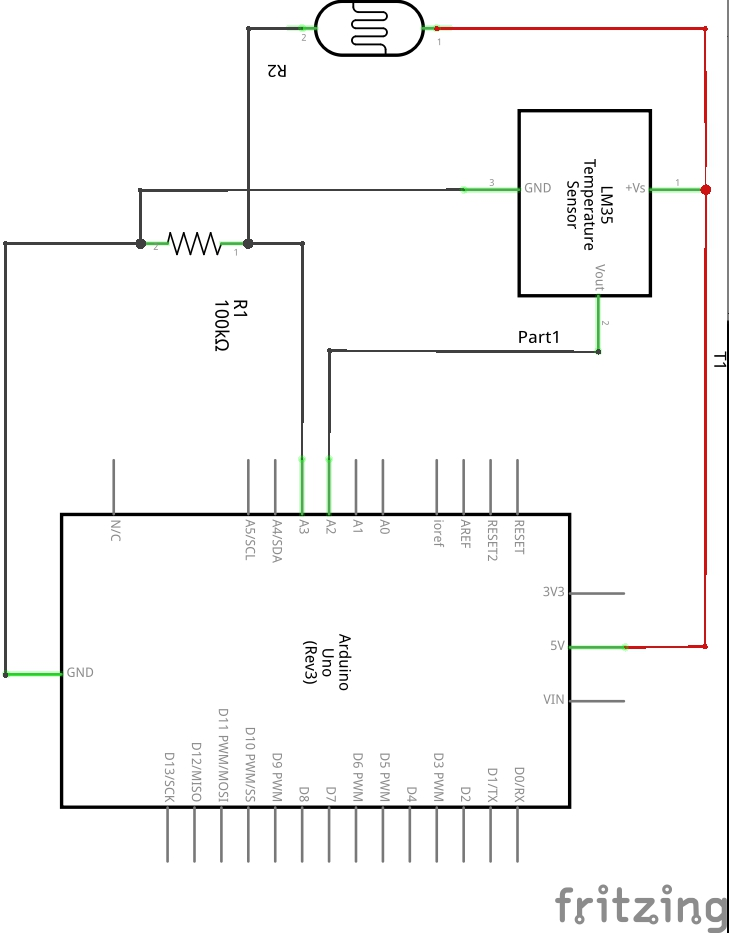
\includegraphics[width=0.9\linewidth,keepaspectratio]{img/luz_temp_sensor_schem.jpg} 

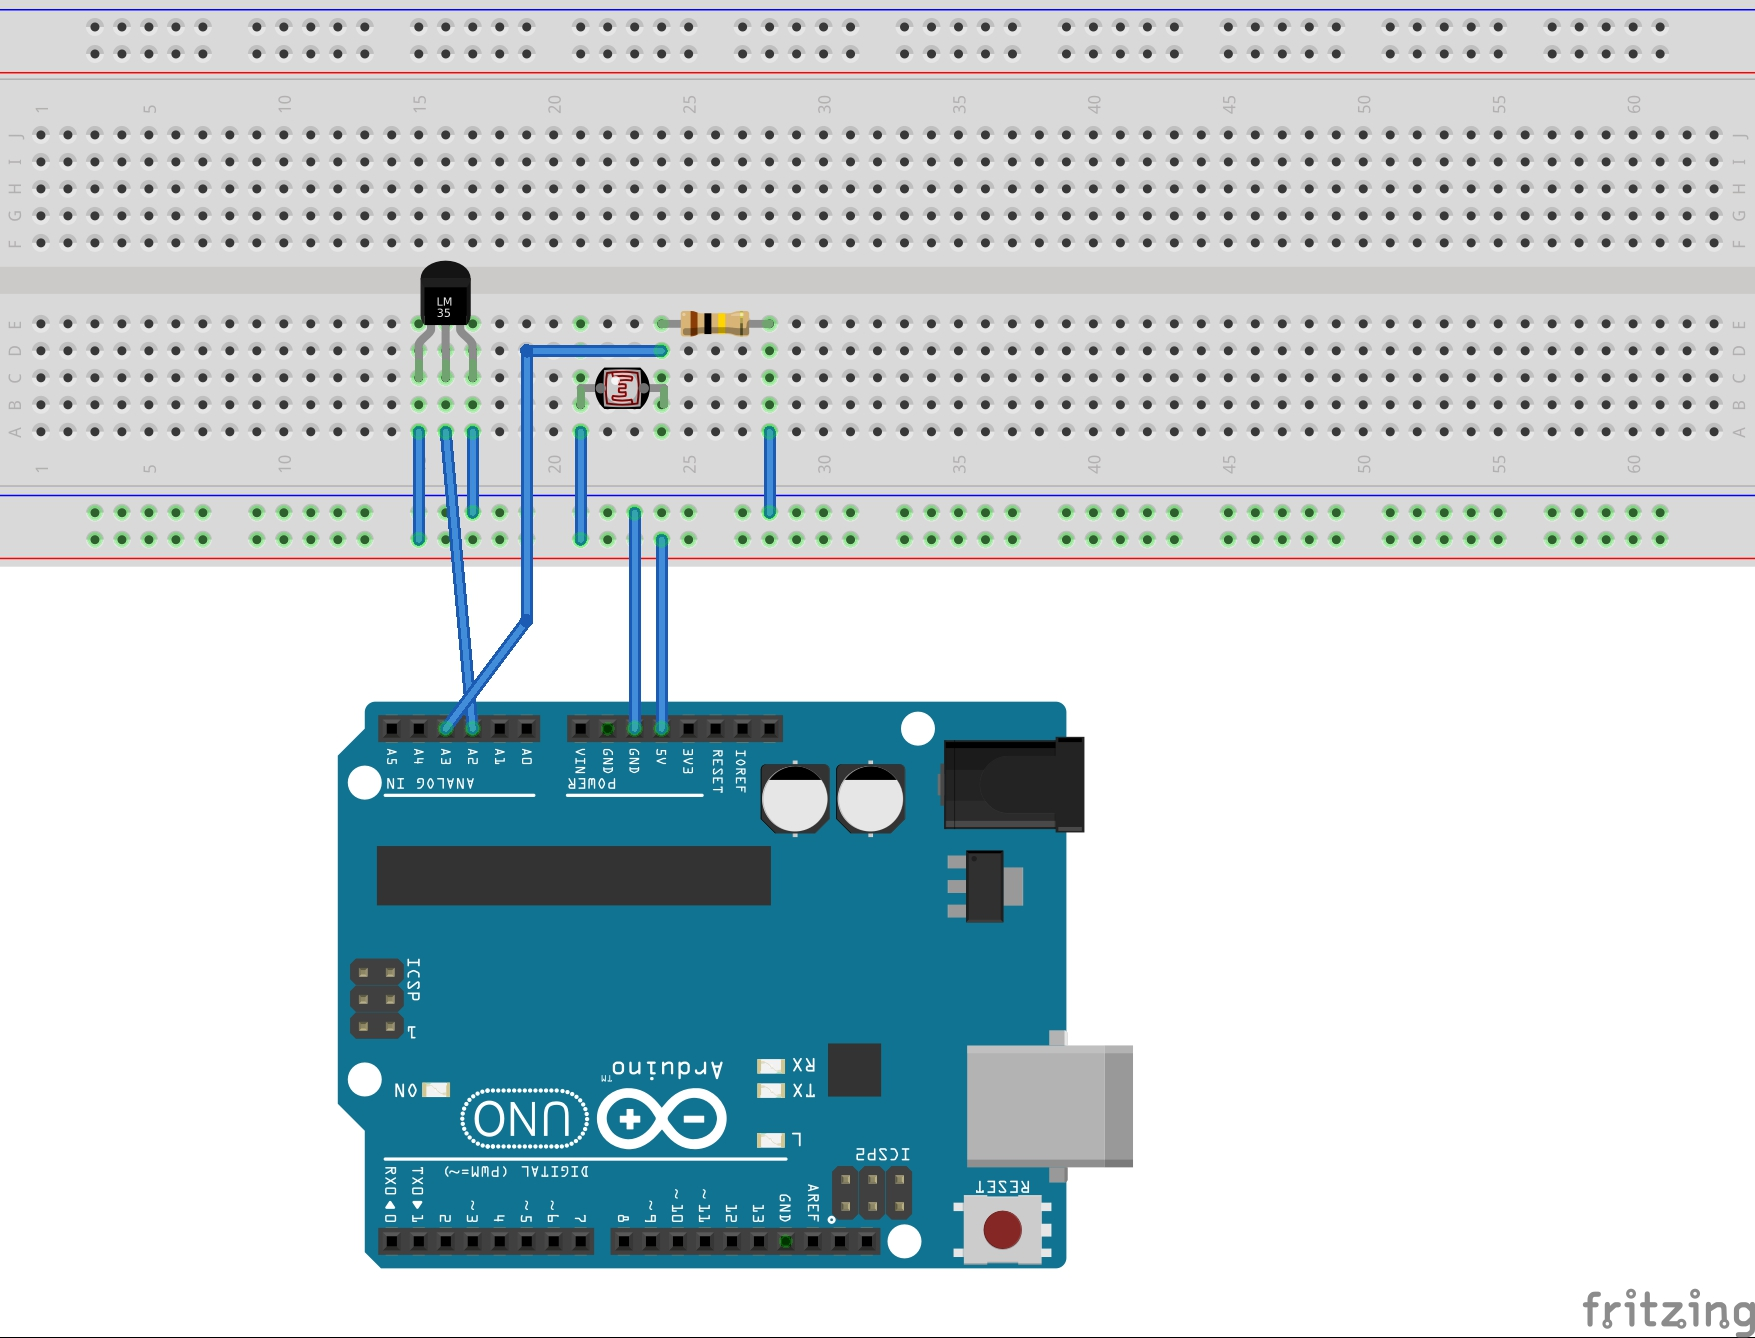
\includegraphics[width=0.9\linewidth,keepaspectratio]{img/luz_temp_sensor_bb.jpg} 

\subsection{Código Arduino}

En este caso el código a usar es bastante mas sencillo: 



\begin{lstlisting}[frame=single]
const int tempPin = A2;
const int lightPin = A3;

void setup() {  
  Serial.begin(9600);
  sleep(1);
}

void loop() {
  //Read temperature pin value
  int tempVal = analogRead(tempPin);
  
  //transform into voltage
  float voltage=(tempVal/1024.0) * 5.0;
	
  //calculate real temperature
  float temperature = (voltage - .5)*100;
 
  //read light pin value
  int lightVal = analogRead(lightPin);
 
  //Create payload with format
  char pld [12];
  sprintf (pld, "#%03i:%03i;",(int)tempVal,(int)lightVal);
 
   //send payload to serial com.
  Serial.println(pld);

  delay(200);//delay for better serial communication
}
\end{lstlisting}

\subsection{Configuración Script-Python}

Una vez tenemos el arduino con el código listo, hay que configurar y arrancar el programa Principal de Python de la raspberryPi

El fichero de configuración mas básico para los datos de nuestro ejemplo sería el siguiente:

\begin{lstlisting}[frame=single]
{
	"control":{
		"address" : "localhost",
		"port": 1883,
		"topic":"master/control",
		"qos":0,
		"control_messages":{
			"reload":"reload",
			"shutdown":"shutdown",
			"status":"status"
		}
	},
	"dbs":{
		"db0":{
			"class_name": "Influx",
			"addres": "localhost",
			"port": "default",
			"db_name": "logger",
			"user": "admin",
			"password": "admin"
		}
	},
	"sockets": [
		{
			"class_name" : "SerialSocket",
			"baudrate":9600,
			"publish" : {
				"parser":"#{0}:{1};",
				"topics":{
					"0":{
				 		"sensortemp": {
							"function":"Raw",
							"samples":1,
							"topic":"arduino/temperatura"
						},
						"temperaturamedia":{
							"function":"Mean",
							"samples":25,
							"topic":"arduino/temperatura/mean",	
							"to_db":{
								"table":"arduino/temperatura/mean",
								"column":"payload",
								"db_id":"db0"
							}
						}
					},
					"1":{
						"sensorluz": {
							"function":"Raw",
							"samples":1,
							"topic":"arduino/luz"
						}
					}
				}
			}, 
			"port" : "/dev/ttyACM0",
			"delay" : 0.1,
			"encode" : "utf-8"
		}
	]
}
\end{lstlisting}

Modificar el ''db\_name'' para ajustarlo al nombre de la base de datos creada anteriormente.

Con esto guardado en un fichero .json (por ejemplo ''arduino.json'') podemos ejecutar el programa principal pasandole como parámetro el nombre del fichero:

\begin{lstlisting}[frame=single]
> python main.py arduino.json
\end{lstlisting}


Ya deberíamos tener los datos publicándose en MQTT con lo que ya podemos ir a Node-Red y trabajar con ellos
o entrar en grafana y utilizar los datos de temperatura media, que son los que hemos decidido guardar. Tal y como hemos visto en el apartado anterior. 

Se invita al lector a probar modificaciones en la configuración del script de pyton y a ''trastear'' con Node-Red  

\end{document}



